\documentclass{beamer}
\usepackage{graphicx}
\usepackage{tikz}
\usetikzlibrary{shapes,arrows}
\usepackage{tikz}
\usetheme{default}
%\usecolortheme{seahorse}
\usepackage{default}

  \setbeamertemplate{footline}[page number]
\setbeamertemplate{navigation symbols}{}
\setbeamertemplate{frametitle}[default][center]
\setbeamerfont{frametitle}{shape=\scshape}

\usepackage{color}
\usepackage{csquotes}

\usepackage{media9}%
\newcommand{\includemovie}[3]{%
\includemedia[%
width=#1,height=#2,%
activate=pagevisible,%
deactivate=pageclose,%
addresource=#3,%
flashvars={%
src=#3 % same path as in addresource!
&autoPlay=true % default: false; if =true, automatically starts playback after activation (see option ?activation)?
&loop=true % if loop=true, media is played in a loop
&controlBarAutoHideTimeout=0 %  time span before auto-hide
}%
]{}{StrobeMediaPlayback.swf}}%


{\title{\textsc{Predictions/Takeaways from Ch. 6 \& 7} \\ \tiny See Barro Ch. 6 and 7}
\author{Trevor Gallen}
\date{}

\begin{document}

\begin{frame}
\titlepage
\end{frame}

\begin{frame}
\frametitle{Some takeaways}
\begin{itemize}
\item The household's budget constraint, plus some obvious intuition about behavior, gives a lot of predictions.
\bigskip
\item A few big, overarching concepts:
\begin{itemize}
\item Income effect:  when you get more money, consume more of all normal goods.
\bigskip
\item Substitution effect:  when something is relatively more expensive, do less of it.  (Do more of things that are relatively cheaper).
\bigskip
\item Leisure and consumption are both normal goods.
\end{itemize}
\bigskip
\item For income effects, what matters is the household's \textbf{permanent} income (lifetime)
\bigskip
\item Know how to draw budget constraints.
\end{itemize}
\end{frame}

\begin{frame}
\frametitle{Budget constraint}
\begin{itemize}
\item Our basic budget constraint (see Barro Ch. 7 or notes for his version) is:
$$w_tL_t+(1+r_t)s_{t-1\rightarrow t}=c_t+s_{t\rightarrow t+1}$$
\item Where, in order, we have:
\begin{itemize} 
\item Labor income $w_tL_t$
\item  Gross capital income (from past savings) $(1+r_t)s_{t-1\rightarrow t}$
\item Consumption expenditures $c_t$
\item Gross capital savings $s_{t\rightarrow t+1}$
\end{itemize}
\item Using savings, these can be combined into a two-period budget constraint (simplifying savings notation and assuming zero savings in the second period):
$$w_1L_1+\frac{w_2L_2}{1+r}+(1+r_t)s_{0}=c_1+\frac{c_2}{1+r}$$
\end{itemize}
\end{frame}

\begin{frame}
\frametitle{Budget constraint}
\begin{itemize}
\item Or we can derive the many-period budget constraint, which says that the net present value of all income must equal the net present value of all expenditures.  
$$\underbrace{\sum_{t=1}^T\frac{w_tL_t}{(1+r)^{t-1}}+(1+r_t)s_{0}}_{\text{Lifetime income}}=\underbrace{\sum_{t=1}^T\frac{c_t}{(1+r)^{t-1}}}_{\text{Lifetime expenditure}}$$
\item This makes clear that a small change in $w_3$, say, makes little difference for your lifetime income.
\bigskip
\item Now we'll think about predictions
\end{itemize}
\end{frame}

\begin{frame}
\frametitle{Theory-Permanent and Transitory Wage Changes}
\begin{figure}
\centering
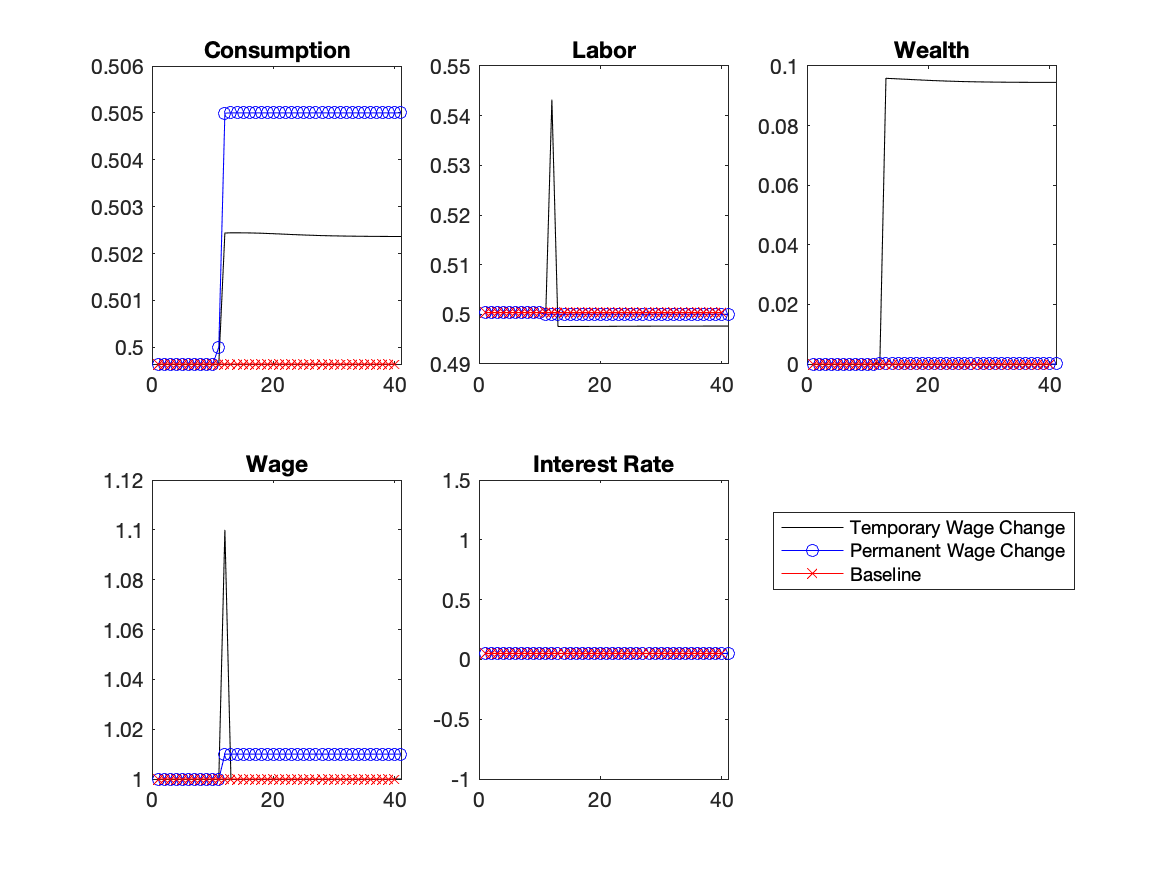
\includegraphics[scale=0.4]{WageChange.png}
\end{figure}
Transitory: work when valuable, then smooth (less labor, more consumption in all periods)\\
Permanent: income and substitution effects largely cancel (no change in labor, more consumption)
\end{frame}

\begin{frame}
\frametitle{Theory-Interest Rate Shocks}
\begin{figure}
\centering
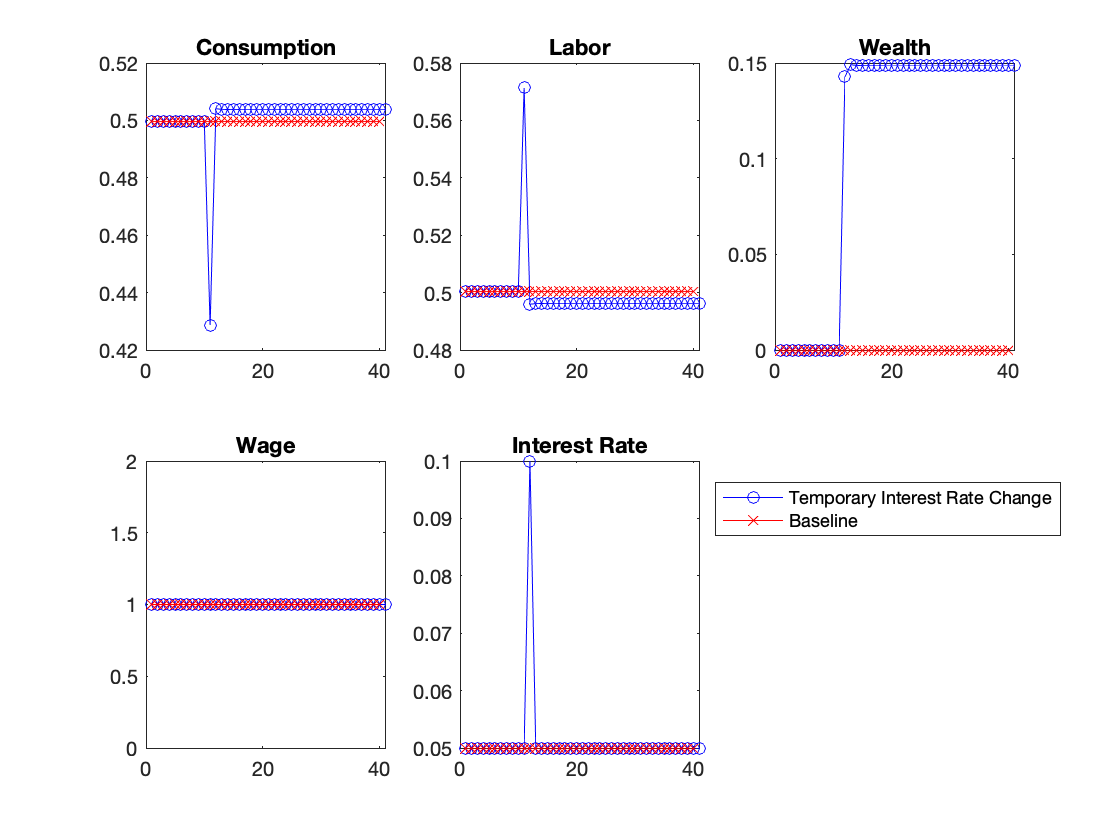
\includegraphics[scale=0.25]{IntChange.png}
\end{figure}
When interest rates rise, put off consumption (and increase labor) to get stream of benefits
\end{frame}

\begin{frame}
\frametitle{Theory-Lump sum transfers }
\begin{figure}
\centering
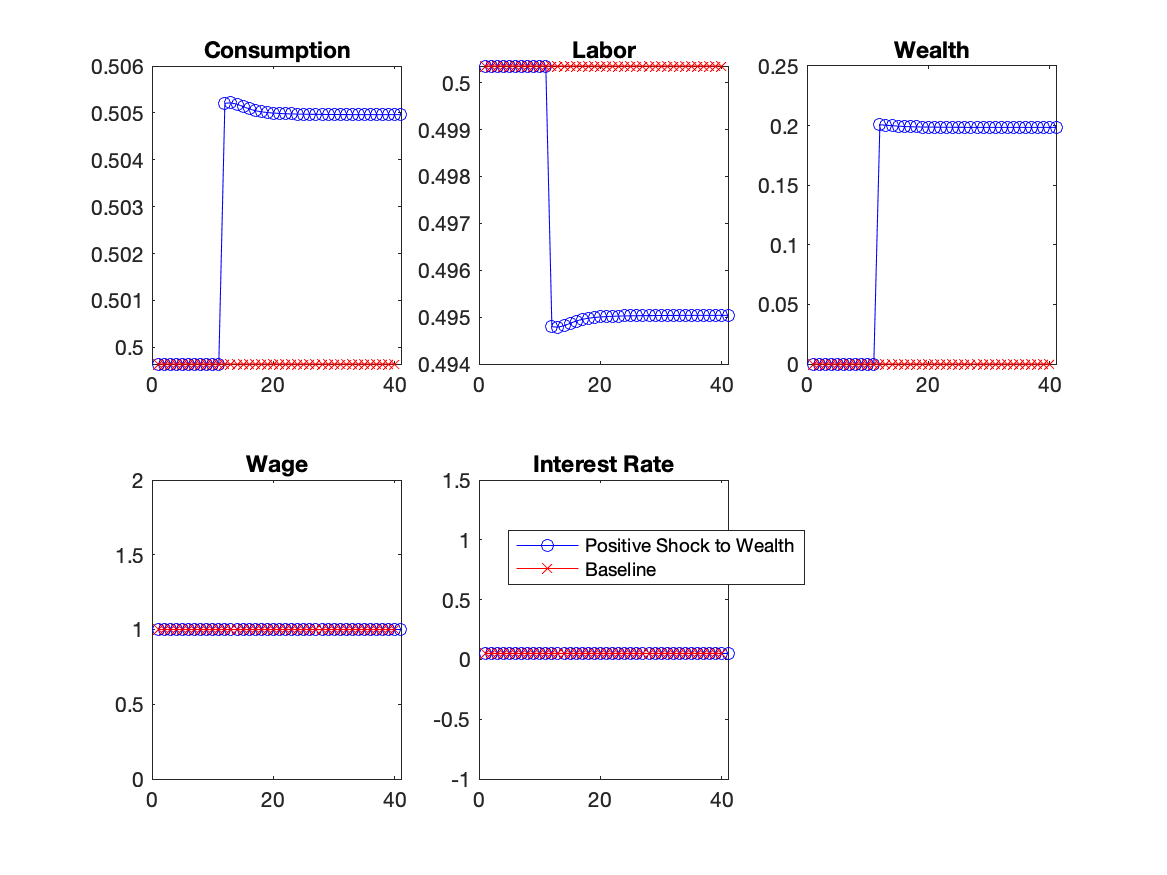
\includegraphics[scale=0.5]{WealthShock.png}
\end{figure}
When shock to wealth (pure income effect) consume more, work less
\end{frame}





\begin{frame}
\frametitle{Prediction 1: Income Timing}
\begin{itemize}
\item \textbf{Prediction} is that it doesn't matter when in our lives we get our income.  If we get it all now, we save it.  If we get it all in the future, we go into debt then pay it off when we get the income.  
\bigskip
\item Data/Experiment:  Alaskans get (or used to get) \$8000/person each year in fourth quarter
\bigskip
\item Result:  Alaskan households had smooth consumptions throughout the year: debt three quarters, save last quarter.
\bigskip
\item Data/Experiment:  Households get sometimes large or surprise tax refunds in U.S.
\bigskip
\item Result:  Households do not see large increases in consumption.
\end{itemize}
\end{frame}


\begin{frame}
\frametitle{Prediction 2: Marginal Propensity to Consume}
\begin{itemize}
\item \textbf{Prediction:}  a large one-time increase in income should not be spent today, but instead smoothed over many periods  
\bigskip
\item Data/Experiment:  Restitution payments to Israeli citizens from Germany ($\approx$ 1 years income).
\bigskip
\item Result:  Total expenditure increased by 20\% of amount (mostly in durable goods, which are savings)
\bigskip
\item Data/Experiment:  WWII veterans got a one-time life-insurance dividend of \$175 (4\% annual income)
\bigskip
\item Result:  Expenditure rose by 35\% of the amount, but again mostly in durable goods.
\bigskip
\item Additional fact:  a large \textbf{permanent} increase in income is met with approximately the same size increase in consumption. 
\end{itemize}
\end{frame}

\begin{frame}
\frametitle{Prediction 3: Anticipated Income Changes}
\begin{itemize}
\item Prediction:  consumption should not change when income is predicted to change
\bigskip
\item Data/Experiment:  Alaskan example (Hsieh 2003) (they don't)
\bigskip
\item Data/Experiment: Income tax refunds (Souleles 1999):  consumption only increases by 10\% of amount 
\end{itemize}
\end{frame}

\begin{frame}
\frametitle{Prediction 3: Anticipated Income Changes}
\begin{figure}
\centering
\bigskip
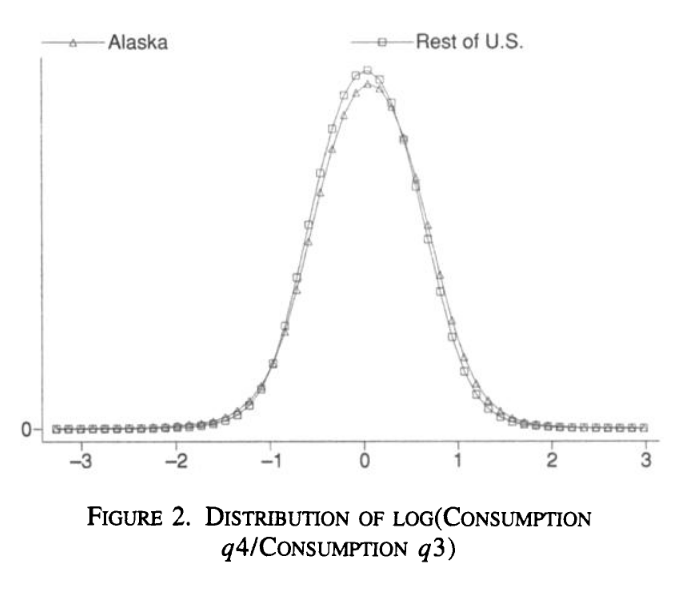
\includegraphics[scale=0.7]{Hseih2003.png}
\end{figure}
\end{frame}




\begin{frame}
\frametitle{Prediction 4: Pure income effects}
\begin{itemize}
\item When households get richer, they should work less  
\bigskip
\item Data/Experiment:  Lottery winners
\bigskip
\item Result:  For every \$1 you get in ``unearned" income, you reduce labor earnings by around \$0.17.
\bigskip
\item Data/Experiment:  Lottery winners (newer paper)
\bigskip
\item Result:  For every \$1 you get in ``unearned" income, you reduce labor earnings by around \$0.50, consumption $\uparrow$ \$0.60
\bigskip
\item Data/Experiment:  Bequests/inheritances
\bigskip
\item Result:  For every \$1 you get in ``unearned" income, you reduce labor earnings by around \$0.09
\end{itemize}
\end{frame}

\begin{frame}
\frametitle{Prediction 4: Pure income effects}
\begin{figure}
\centering
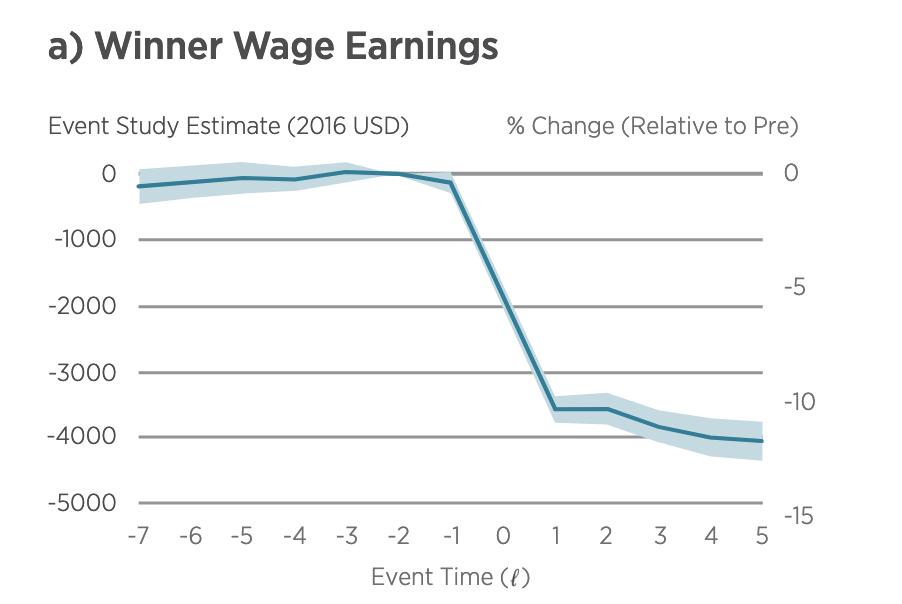
\includegraphics[scale=0.6]{Mogstad.png}
\end{figure}
\end{frame}




\begin{frame}
\frametitle{Prediction 5: Interest Rates}
\begin{itemize}
\item Another prediction we have is that a higher interest rate reduces current consumption \textbf{compared to} future consumption $c_2/c_1$.  
\item Also, Higher interest rates mean households should work now
\bigskip
\item Data/Experiment:  Longitudinal data on U.S. household purchases
\bigskip
\item Result:  A 1 percentage point increase in the interest rate increases $c_2/c_1$ by about 0.5 percentage points/year.
\bigskip
\item Data/Experiment:  Aggregate economy
\bigskip
\item Result:  A 1 percentage point increase in the interest rate increases $c_2/c_1$ by about 0.3 percentage points/year.
\bigskip
\item Data/Experiment:  Data on annual interest rates
\bigskip
\item Result:  A 1 percentage point increase in the interest rate increases $L_2/L_1$ by about 0.2-0.6 percentage points/year.
\end{itemize}
\end{frame}


\begin{frame}
\frametitle{Prediction 6: Permanent wages changes}
\begin{itemize}
\item When households get permanently higher wages, it's unclear what they should do, income and substitution effects offset  
\bigskip
\item Data/Experiment:  Long-run wage increases in U.S.
\bigskip
\item Result:  Little change in long-run labor
\end{itemize}
\end{frame}

\begin{frame}
\frametitle{Theory-Lump sum transfers }
\begin{figure}
\centering
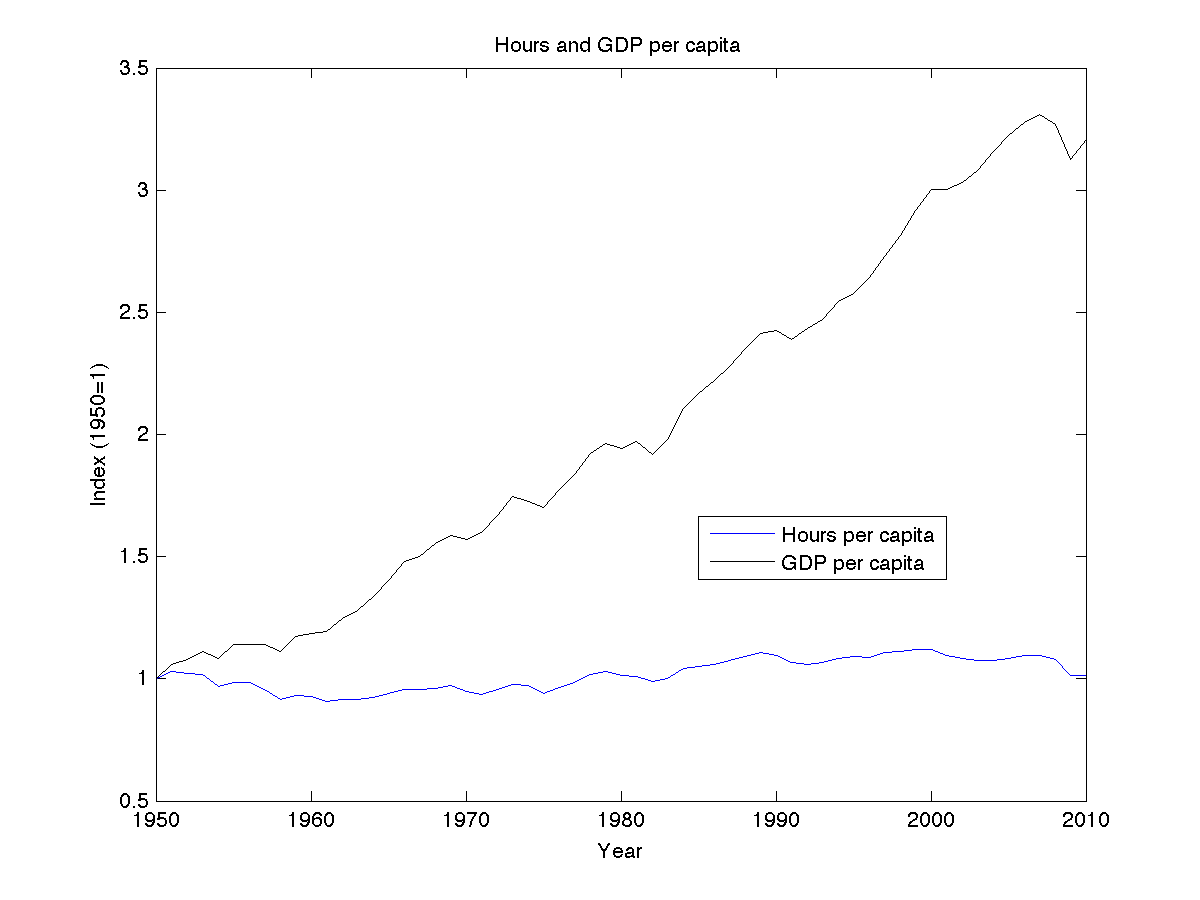
\includegraphics[scale=0.5]{Figure10.png}
\end{figure}
Even as wages ($\Delta$ ln GDP$\propto \Delta$ ln w) increase, $L$ stays the same
\end{frame}



\begin{frame}
\frametitle{Prediction 6: Temporary wage changes}
\begin{itemize}
\item When households get temporarily higher wages, income effects are small but substitution effects are big: work more
\item When wages will be higher in the future, move labor to the future
\bigskip
\item Data/Experiment:  Data on employee expectations about wages
\bigskip
\item Result:  An increase in expectations about $w_2/w_1$ by 1 percentage point increased $L_2/L_1$ by 1 percentage point.
\bigskip
\item Data/Experiment:  Exxon Valdez spill
\bigskip
\item Result:  A temporary increase in real wage rates by 1\% increased hours worked per week by 2\%
\end{itemize}
\end{frame}


\end{document}


